\chapter{Variable selection pressure}
In the original paper, Fernando et al. used a tournament search algorithm for optimizing the modules used for a given task. This algorithm was selected on the basis that it fills the role of simplest possible 'agent' for path-selection, one which can be considered a unit of evolution.  The tournament implementation fits this description as a 'unit' because of the tournament size used. Within one generation, the total change in the population is one genotype being replaced with another from the same population and subjected to mutation under some probability. Building on the previous set of experiments where the conclusion can take form as an argument in favour of a high exploration rate during path-search, we would expect a tournament of size two to yield modules with high transferability and a high number of reuse. 
In these experiments, this will be tested by manipulating the selection pressure during the tournament search. Questions addressed in this section is: 
\begin{itemize}
    \item How would different evolutionary algorithms influence outcomes in training a PathNet structure on multiple tasks?
    \item What evolutionary strategies make the most sense in the scheme of training an SNN?
    \item How would a changing selection pressure affect learning? 
\end{itemize}

\section{Description}\label{Search-datasets}
\subsection{Data-sets} \label{Search-experiment:Datasets}
To address these questions a trial of different searches have been applied to a PathNet structure for a selection of tasks. As with the first-path experiments, the search algorithms will be applied to image classification tasks. Building on what we learned with regards to task difficulty, two different data-sets have been selected, and the different tasks will be derived from this data. The tasks will be ordered by assumed difficulty to follow a gradual learning mentality. 


\begin{enumerate}
    \item MNIST subtasks
    \begin{enumerate}
        \item Digits 0, 1, 2, 3 and 4
        \item Digits 5, 6, 7, 8 and 9 
    \end{enumerate}
    \item Full MNIST classification
    \item Cropped SVHN subtasks
    \begin{enumerate}
        \item Digits 0, 1, 2, 3 and 4
        \item Digits 5, 6, 7, 8 and 9 
    \end{enumerate}
    \item Full cSVHN classification
\end{enumerate}

It was shown during the first-path experiments that task 1a and 1b is not of the same difficulty level, however, within this context we will consider the training amount needed to reach a satisfactory accuracy level is similar enough for these tasks to be grouped together.  The natural progression from a full MNIST classification to a SVHN is though to increase the incentive for module reuse, even though if the SVHN task will have to learn to ignore distractions in the images (see SECTION ON SVHN) that the MNIST classifiers does not have to deal with. The difference in image-dimensions have been addressed in \ref{Search-implementation}.

As mentioned in *SECTION ON SVHN* there are two formats to the SVHN set, one of variable image resolutions, and one that mimic the MNIST set in static square size called cropped SVHN (cSVHN). cSVHN is selected for these experiments in order to use a constant input size to the pathnet, and within the larger set of cSVHN images, a subset described as containing "somewhat less difficult samples".
To increase the number of tasks, the rest of the data in SVHN could be used, and noise could be added to the images to increase the task difficulty artificially. 

For both the MNIST and cSVHN set, the amount of training data have been limited to 10000 training samples and 4000 validation samples. Of these samples, MNIST have an fairly even distribution on each class while SVHN have an imbalance in the class distribution. Since the samples used are randomly selected before each experimental run, the probability of select one sample from a given class can be derived from the total amount of samples in that class (see SECTION ON SVHN  for the exact number of samples in each class).
%BENFORDS LAW 

Each experimental run will apply a searching scheme to find an optimal path in a gradually increasing knowledge base within a PathNet. This means tasks 1a always will be learned in a module set of only initialized weights and no previous knowledge. It is assumed that with a different ordering in tasks, other  accuracy and training results would have been reached, but as this tells us more about the tasks selected than it does about the search algorithms used, and as each experimental run is significantly more time consuming than in the first-path experiments, this will not be attempted here. It is considered that this reversing of subtasks within a data-set partition could be used as an simple, if time consuming and crude analysis tool.

\subsection{Algorithms}\label{Search-experiment:Algorithms}
The different versions of tournament search explored here have been divided into three groups: 
\begin{enumerate}
    \item Constant selection pressure
    \begin{enumerate}
        \item Tournament size 2
        \item Tournament size 25
        \item Tournament size 3 + recombination
    \end{enumerate}
    \item Changing selection pressure between tasks
    \begin{enumerate}
        \item Low to high pressure: 2, 5, 10, 15, 20, 25
        \item High to low pressure: 25, 20, 15, 10, 5, 2
    \end{enumerate}
    \item Dynamic selection pressure
    \begin{enumerate}
        \item Gradual change from 2 to 25 over all generations
        \item Gradual change from 25 to 2 over all generations
    \end{enumerate}
\end{enumerate}
In total, the seven tournament algorithms are used 10 times each within a reinitialized PathNet structure to train on all tasks discussed in \ref{Search-experiment:Datasets}. Between algorithms, the only variable change is the tournament size and replacement method within each tournament. All algorithms except 1c use a winner-replace-all scheme where the mutation of the strongest paths genome replaces each of the loosing contenders. In algorithm 1c, three contenders are selected randomly from the population and evaluated. The two strongest genomes are labeled parents and (starting with the winner) takes turns copying their layers to the offspring. The offspring is then subject to some mutation under the same probability as every other algorithm, and replaces the loosing genome of the three selected. 
\begin{figure}[h]
    \centering
    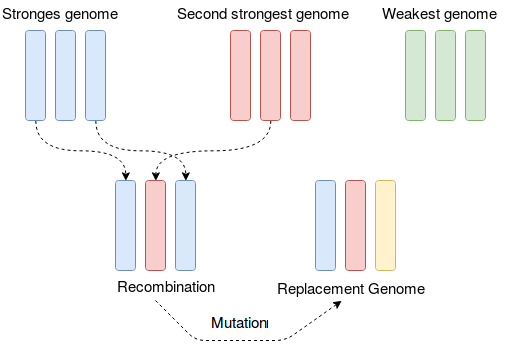
\includegraphics[width=0.8\textwidth]{Chapters/Experiments/search_algo/figures/Recombination_algorithm.png}
    \caption{Visualization of the recombination in algorithm 1c. In a three layer PathNet, the first and last layer in the recombination would be layer one and three in the winning genome, while layer two would stem from the second strongest genome. After a mutation of the recombination, the new genome replaces the loosing contender. Each color represents one genome from the tournament and yellow represents a mutation.}
    \label{fig:search.recombination_algorithm}
\end{figure}

Algorithm group two consists of two algorithms where the tournament size is changed between each task. This means algorithm 2a uses tournament size 2 for task 1a, task 1b uses tournament size 5 and so on until the last task of full cSVHN classification which uses tournament size 25. In algorithm 2b, this order of tournament sizes is reversed. It is expected that in visualization of metrics where a population average is calculated, such as training accuracy, an algorithm with high selection pressure will have abrupt value changes from one generation to the next. Low selection pressure would then give a more gradual change in such values. A change between these two curve types should be prominent or algorithms 2a and 2b.

Algorithms 3a and 3b have its selection pressure changed during each search for optimal paths. This means each algorithm behave the same for each task, which algorithms 2a and 2b did not. The change in selection pressure is gradual which means between tournament sizes 2 and 25, each tournament size is used about 4 times for a limit of 100 generations. It is obvious that an even distribution of tournament sizes on each generation is not possible when using a threshold accuracy as search termination, which is one reason searches in these experiments are limited by number of generations instead. 

\subsection{Metrics}\label{Search-experiment:Metrics}
Due to the experiment complexity and number of tunable hyperparameters there are a large number of search effects and attributes that could be investigated, so limitations have been introduced on which metrics are being addressed. 

As with the first-path experiments, module reuse between tasks will be an important metric. This number is highly effected by stochastic processes such as initialization of populations, mutation probability, layer sizes, path sizes and so on, but it is also the most intuitive and clear way to measure the transferability of modules. An assumption used behind this metric is that modules are able to contain some form of "memetic"\footnote{Memetic is used here to describe a quantification of knowledge in the same way "meme" is used by Richard Dawkins\cite{selfishGene} to describe a unit of cultural knowledge} unit knowledge. In this multi-task scenario, reuse can occur across multiple tasks, but focus will here be put on the total number of modules reused instead of separating the reuse across tasks. This is because if the effect on reuse between each search algorithm is small, the stochastic noise in reuse on between two tasks is not as descriptive of how an algorithm affects learning as with the total number. 

This reuse can indirectly be viewed by viewing the total number of modules used for all tasks. This total capacity use is both a result of the reuse of modules and the module size. Which means capacity could be used as a measure of how "effective" the learning under a search algorithm is. By using few modules in each task and reusing a high number of modules from previous tasks, little new parameter optimization have to be done. This effective parameter use would possible reduce the overall validation accuracy so in order to visualize the effectiveness of training, total number of training units applied to each module in each path would be a useful metric. 

To confirm the ordering of algorithms on the exploration/exploitation scale, a population diversity metric will be calculated. Morrison et al.\cite{populationDiversity} described the pair-wise Hamming distance as one of the most commonly used measures of distance in genotypic space, and is what will be used here to calculate a populations diversity as one scalar metric. In implementation, this algorithm\ref{eq:Hamming} is counting the number of genomes in all pairs of genotypes which is not identical. Another description is the edit distance between two binary genomes. 
\begin{equation}
    \label{eq:Hamming}
    H=\sum_{j=1}^{j=P-1}\sum_{{j}'=j+1}^{{j}'=P}\sum_{i=1}^{i=L}\left |y_{ij}-y_{i{j}'}\right |
\end{equation}

where y is a genotype, P is the population size and L is the number of genomes in a genotype.

A problem with using a pairwise Hamming distance is that the number of computations is quadratic with the size of P. Meaning the computational time is quite long, but since this metric is only to be calculated once when experimentation is completed, the restriction this puts on the experiment is negligible. However, a suggested alternate way of calculating population diversity on the basis of edit distance is by calculating the mean edit distance from every genotype to a \textit{centroid} genotype where the centroid is the average genotype in a population, and its i-th element can be given as  
\begin{equation}
    \label{eq:centroid}
    \varphi_{i}=\tfrac{1}{P}\sum_{j=1}^{P}y_{ji}
\end{equation}
Using this vector that can be calculated linearly with respect to P, a diversity metric \(\Delta\) can be calculated as 
\begin{equation*}
    \Delta = \tfrac{1}{P}\sum_{j=1}^{P}\sum_{i=1}^{L}\left | \varphi_{i}-y_{ji} \right |
\end{equation*}

\begin{equation}
    \label{eq:homemade diversity}
    \Delta = \tfrac{1}{{P}}\sum_{j=1}^{P}\sum_{i=1}^{L}\left | (\tfrac{1}{{P}}\sum_{{j}'=1}^{P}y_{{j}'i})-y_{ji} \right |
\end{equation}
While it is obvious that calculation time grows linearly for larger population sizes and the computational requirements for large experiments are greatly reduced, the pair-wise Hamming distance is a tried and tested diversity metric, and is what will be used to describe the change in diversity between generations and algorithms. 

During a search for an optimal path as solution to a given task, the total training effort spent on the task is spread across the modules available for training. This means when the search is terminated and the optimal path have been locked to future back propagation, most of the updated parameters are lost due to the re-initialization of PathNet. While total computational efficiency is not something addressed in this thesis, the ratio of used training effort to the total training spent on a task is an interesting metric. This ratio is highly dependent on how quickly a population converges to one optimal path. In scenarios where this occur fairly early on in the lifetime of the search, every subsequent generation performs training where almost all is along the optimal path. We would therefore expect algorithms with a high selection pressure to be placed high in a ranking of useful training. See \ref{Search-implementation} for description of a training unit. 

\section{Hypothesis}\label{Search-hypothesis}
The expectations for these experiments were heavily influenced by the results in the first-path experiments. When the training algorithms are viewed in a simplified context of only "exploration vs exploitation", we can place them on a scale between these extremes and discuss expected outcomes from each end of the spectrum. In this context, the Pick+Search learning scheme used in the first-path experiments would fall on the exploitation.

During a search, a given algorithm would have a population with consistently high diversity until the population converges to an optimal path. This convergence rate, and therefore also population diversity, is determined by which end of the exploration/exploitation spectrum we select our algorithm from. Since we limit ourselves by only changing the tournament size, we would expect a lower tournament size to lead to a low convergence rate and high diversity. This is a natural assumption to make considering the maximum change that occur in the population from one generation to the next. A tournament search with tournament size two has such a low selection pressure that from one generation to the next, only one instance of genotypic change is applied the the population\footnote{This is when the weakest genotype is replaced by the winner of the tournament}. The number of generations until the population have converged to one optimal path would therefore be higher under such a search, than a search where the selection pressure is considerable higher. 

A high selection pressure means strong phenotypes are favoured during the search. The algorithm would after one generation have a significant portion of its population genetically identical, ignoring possible genotypic traits caused by mutations. In the search context of finding an optimal path in a PathNet structure, evaluating a lot of similar paths to rank their fitness would lead to training the same modules multiple times. The next generation would then have a disproportionate fitness scores for some paths which would cause them to have a higher likelihood of winning the next generations tournament, and therefore quickly take control of a population by out performing all other paths. In such a scenario, the population have converged before other paths would have had time to adapt to pretrained modules interfaces, and the advantage PathNet brings with module transferability have been reduced, if not lost.  

For the locked tournament sizes the expectations are that high selection pressure causes high convergence and low module reuse between tasks. The low reuse would again cause more of the total number of modules in the PathNet to be locked after all tasks are learned. What the pressure would mean for validation accuracy is highly dependent on what tasks are learned, and from which domains they are selected. 
The opposite is true for the searches with a small tournament size. The low convergence leads each module to be trained in multiple permutation of PathNet subsets, and therefore also more transferable than modules trained during high selection pressure. If the searches are limited by the number of generations, and not by a threshold training accuracy, it would not be a surprise if the high tournament sizes yields paths with a higher validation accuracy for each task than those searches with low selection pressure. This is because each generation contain more effective training when there are more genotypes in the tournament. 
Not to be forgotten is the fact that all paths in one generation have the same final task specific layer.  Since this is shared across all paths, the high tournament sizes leads to orders of magnitude more training in the final layer for high selection pressures. For each generation, the final layer is trained once for each genotype being evaluated. Meaning after a hundred generations, it have been trained 2300 times more for a search with tournament size of 25 versus a tournament size of 2. 

% Variable tournament size between tasks: Dont know how it will affect
% Dynamic tournament size during search: Dont know

In addition to the static tournament sizes with a winner-replace-all crossover scheme, a search with recombination is tried together with tournament size three.  This should give a selection pressure even lower than that of tournament size two. From one generation to the next, there is still only one genotypic change in the population, but where the normal tournament search replace the loosing genotype with the winner, a recombination of the two strongest phenotypes replaces the weakest genome\footnote{With some additional mutation}.  Another way to view the step from tournament size two to size three with recombination is one with focus on the genome in the offspring that takes the weaker paths place in the population. Given the recombination scheme, it can be seen as a copy of the tournament winner, but with a strong mutation probability that is scaled down during the search. This down scaling comes from the convergence of the population. When the diversity is reduced, more and more paths will have a similar subset of PathNet. When selecting two paths with the same modules, the recombination will yield a path identical to both parents. So as a population grows closer to converging to an optimal path, it will consist of similar genomes and each recombination will give offspring closer to the population median than it would in a diverse population. 

% Some illustration of exploration vs exploitation: Hypothesis figure of where i think algorithms falls


% High tournament size: 
%% High convergance
%% Lots of training in optimal path
%% Low reuse
%% Diversity is high in the beginning when the modules still havent adapted to each others interface. => Dont take advantage of pretrained modules

% Low tournament size
%%  Lower convergance
%% Less return on investment in training
%% more ruse
%%% As effect of more reuse -> less used capacity in the pathnet
 
\section{Implementation}\label{Search-implementation}
The PathNet structure used for these experiments had three layers of 20 modules in each where each path may contain one, two or three modules in each layer. The 20 modules were selected to make sure there would be a a non-zero probability of selecting only empty modules for all tasks, even if all optimal tasks contained the maximum number of modules without any module overlap between tasks.

As with the refined first-path experiments, only convolutional modules were used, but with two channels each instead of the one in first-path. To verify, a random path with these hyper-parameters were created and applied to the task of full cSVHN classification and was able to reach a satisfactory performance within a reasonable training time. All modules use a ReLU-activation function and the Adam optimizer were used during back propagation with a learning rate of 0.0001. 

Each convolutional module also includes a batch-normalization operation and the last module ends in a max-pooling before the output is flattened and passed through the final unique classification layer. 

As there is a resolution difference between the cSVHN set and MNIST, an additional preprocessing step were applied to the MNIST set. A 2 pixel border of zeros were added to change the dimensions from 28x28 to 32x32. cSVHN images has three-channels of RGB values so the single channel of padded MNIST images were repeated in every color-channel to reach the final dimensions of 32x32x3.  

\begin{figure}[h]
    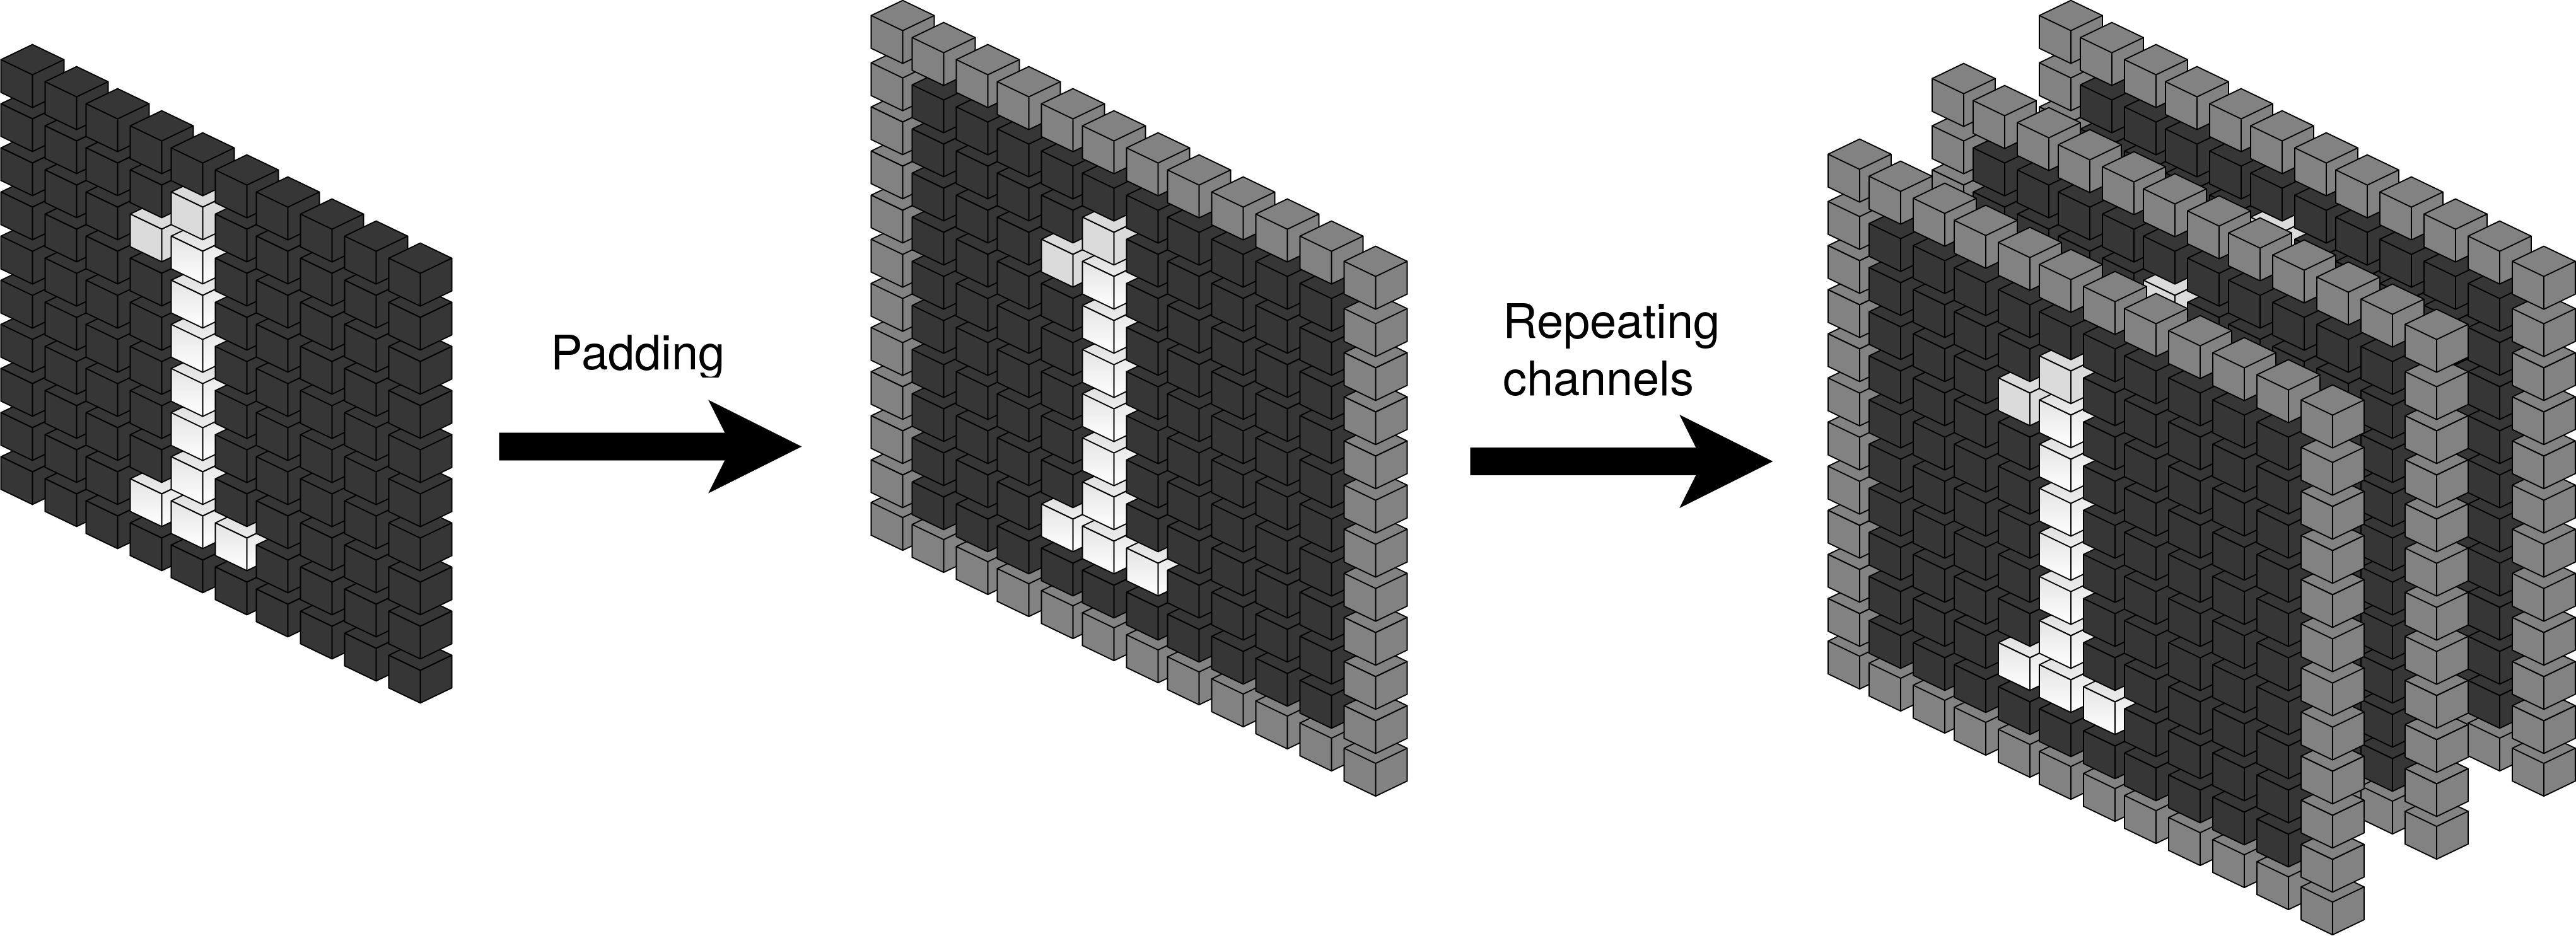
\includegraphics[width=\textwidth]{Chapters/Experiments/search_algo/figures/MNISTpadding+repeating.png}
    \caption{How MNIST is adapted to have same dimensions as cSVHN. Illustration use dimensions 12x12x3 while cSVHN and adapted MNIST use 32x32x3}
    \label{fig:MNISTpadding}
\end{figure}



%Hyperparameters to search
%%% Why 100 generations locked instead of acc-threshold?
%%% 
%Hyperparameters to pathnet




\section{Results}

\begin{figure}[h]
    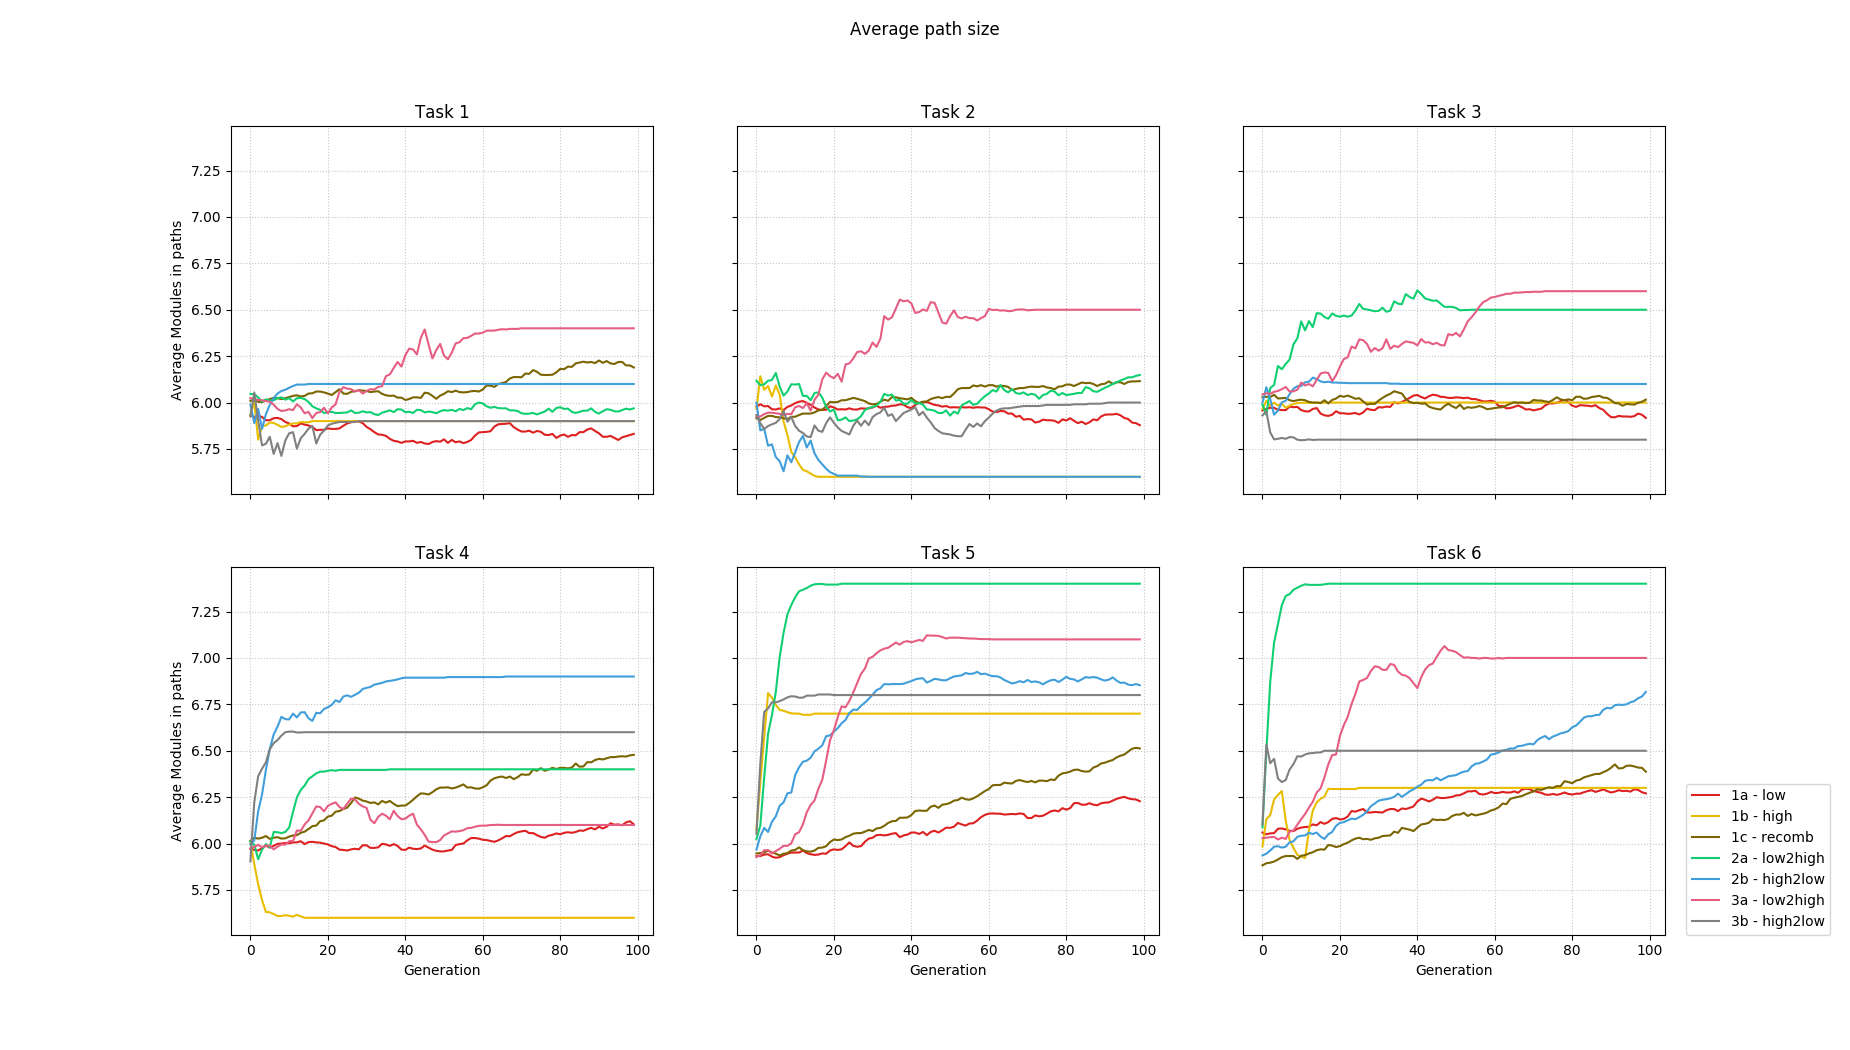
\includegraphics[width=\textwidth]{Chapters/Experiments/search_algo/figures/Average_path_size.png}
    \caption{Change in average path size for each tournament scheme plotted for each task.}
    \label{fig:search.avg_path_size}
\end{figure}

\begin{figure}[h]
    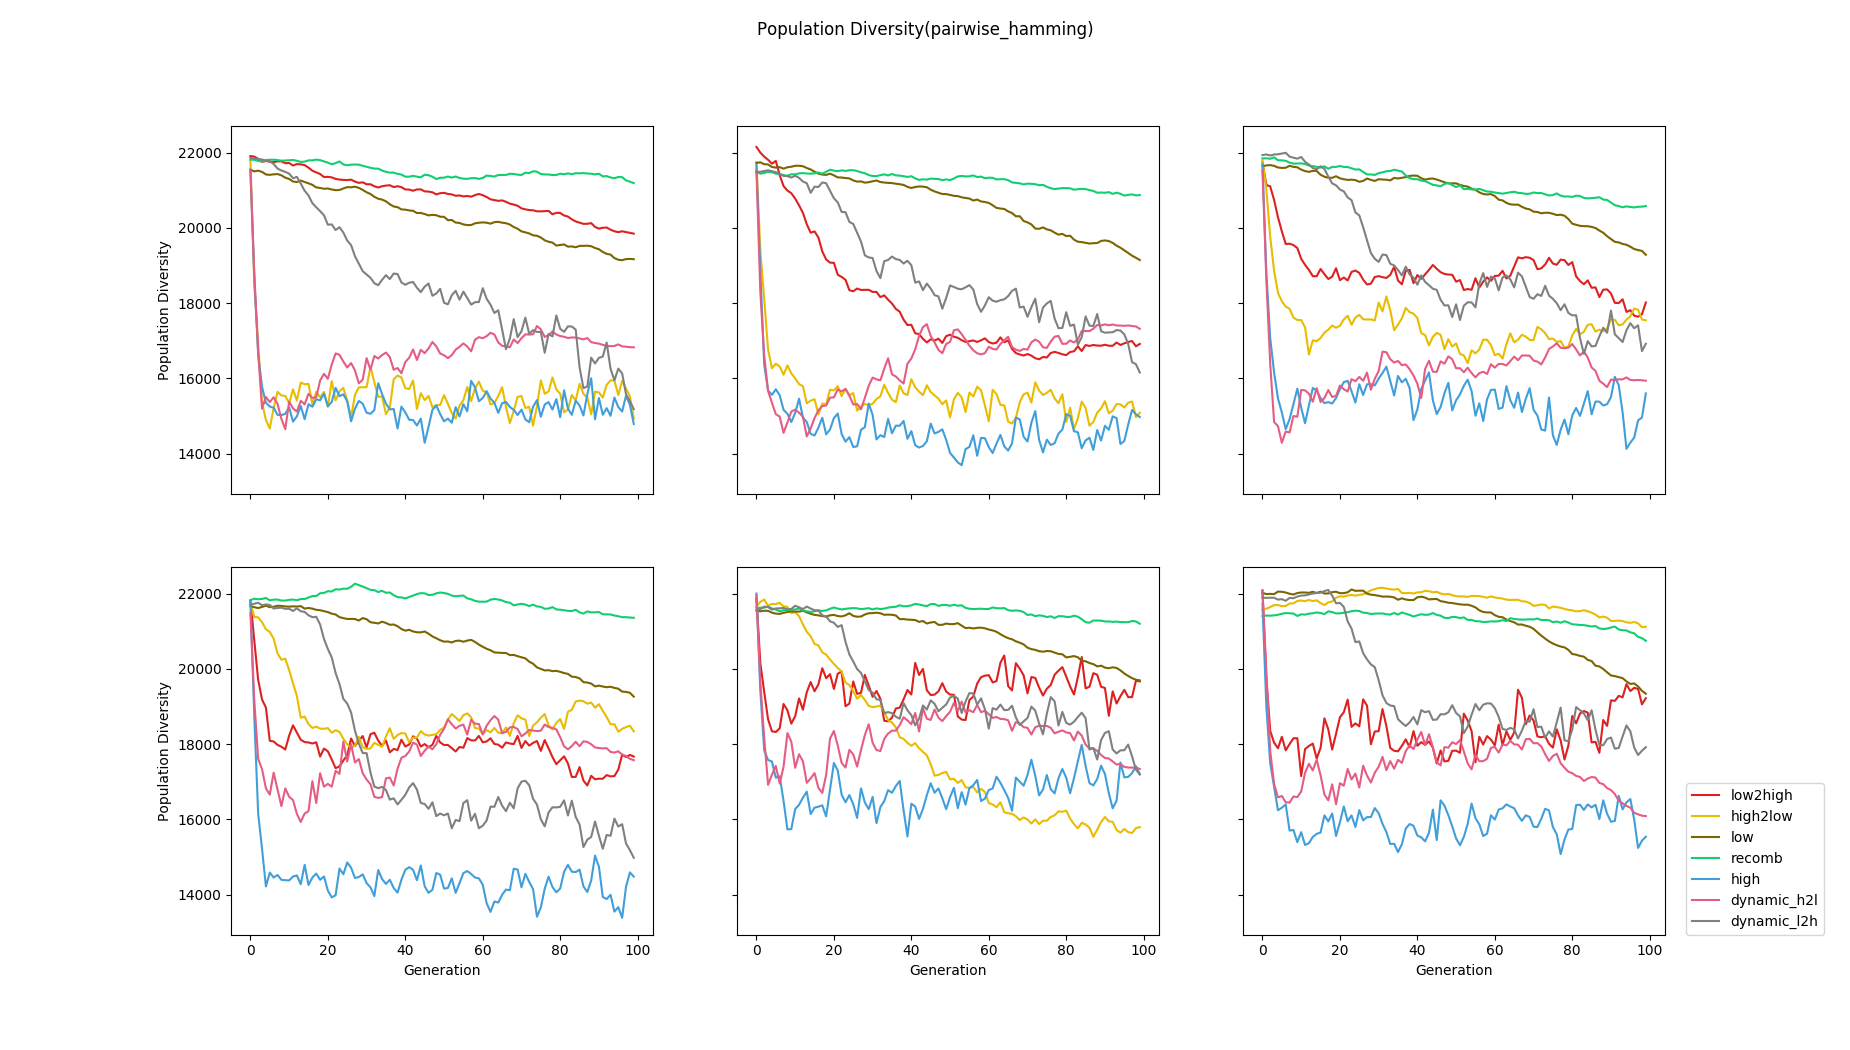
\includegraphics[width=\textwidth]{Chapters/Experiments/search_algo/figures/Average_population_diversity_pairwise_hamming.png}
    \caption{The average pairwise Hamming distance within each generation is used as a measure for population diversity. Each plot is (in order left to right) the different task.}
    \label{fig:search.diversity}
\end{figure}

\begin{figure}[h]
    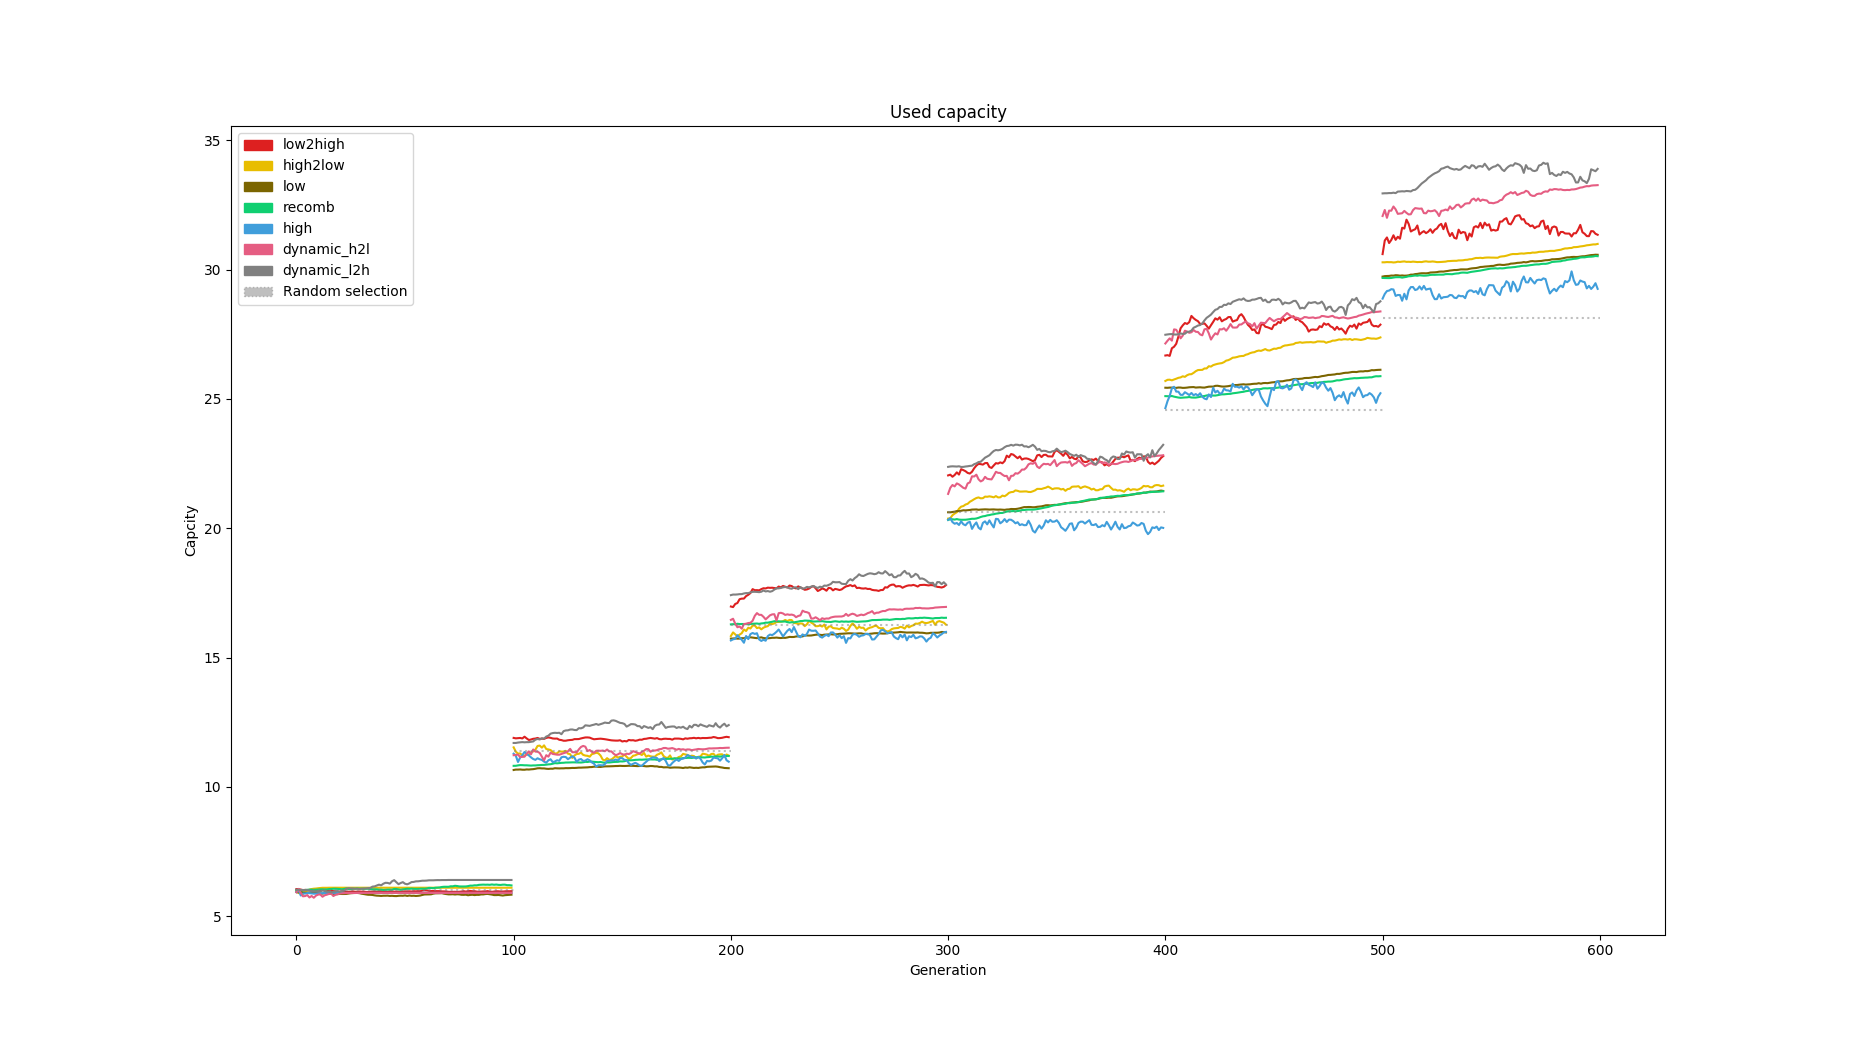
\includegraphics[width=\textwidth]{Chapters/Experiments/search_algo/figures/Capacity_pr_generation.png}
    \caption{}
    \label{fig:search.capacity}
\end{figure}

\begin{figure}[h]
    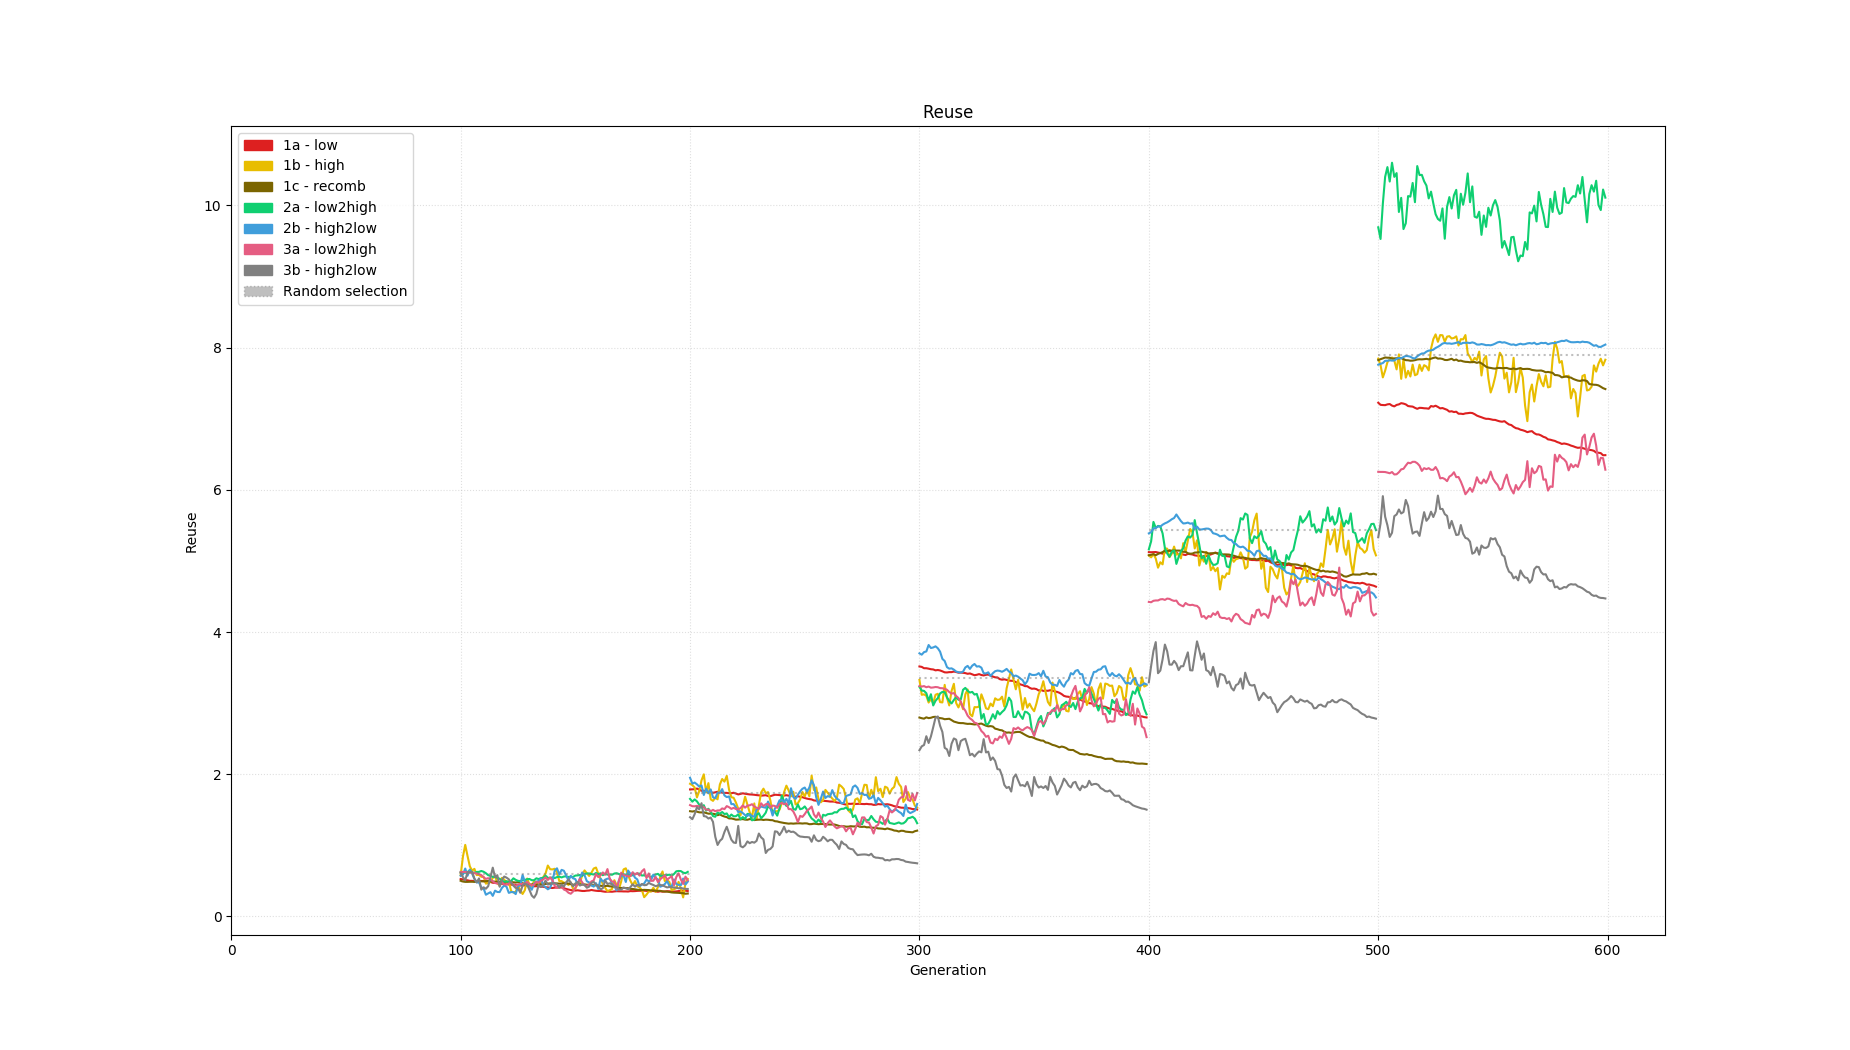
\includegraphics[width=\textwidth]{Chapters/Experiments/search_algo/figures/Module_reuse_pr_generation.png}
    \caption{}
    \label{fig:search.reuse}
\end{figure}

\begin{figure}[h]
    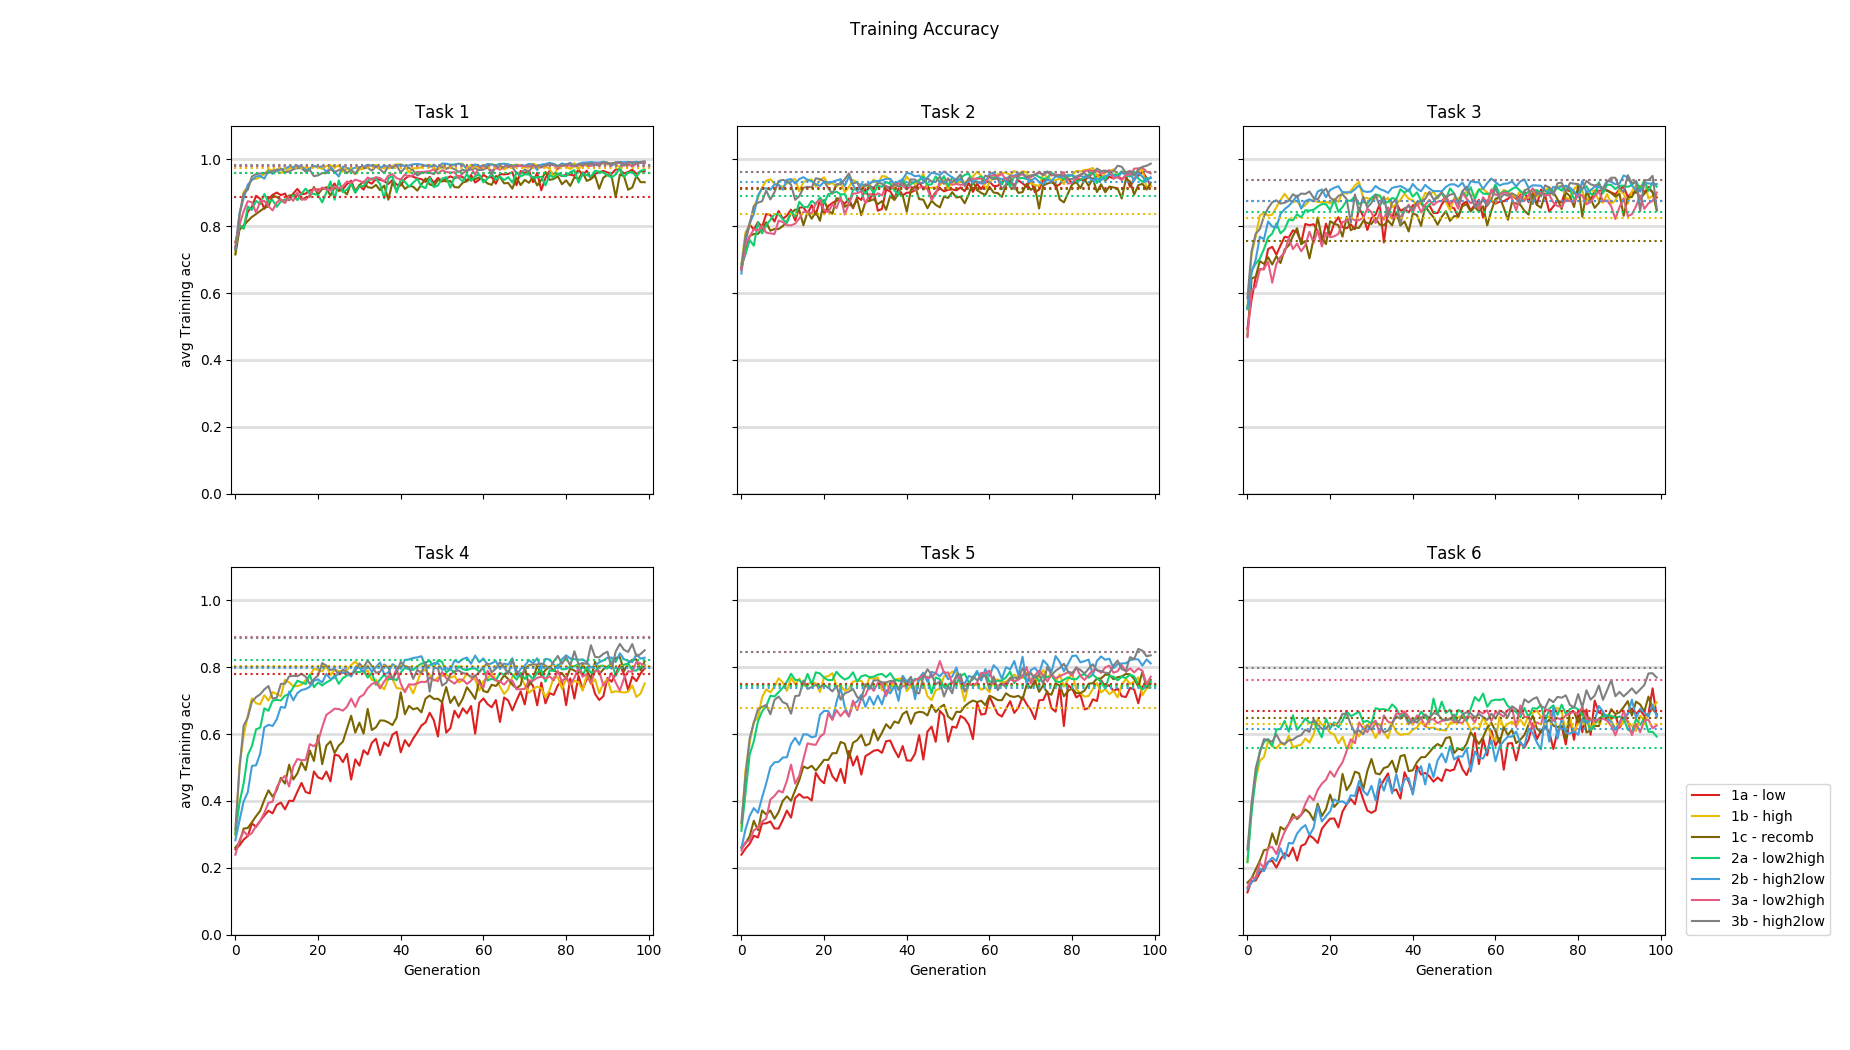
\includegraphics[width=\textwidth]{Chapters/Experiments/search_algo/figures/Training_accuracy.png}
    \caption{}
    \label{fig:search.accuracy}
\end{figure}

\begin{figure}[h]
    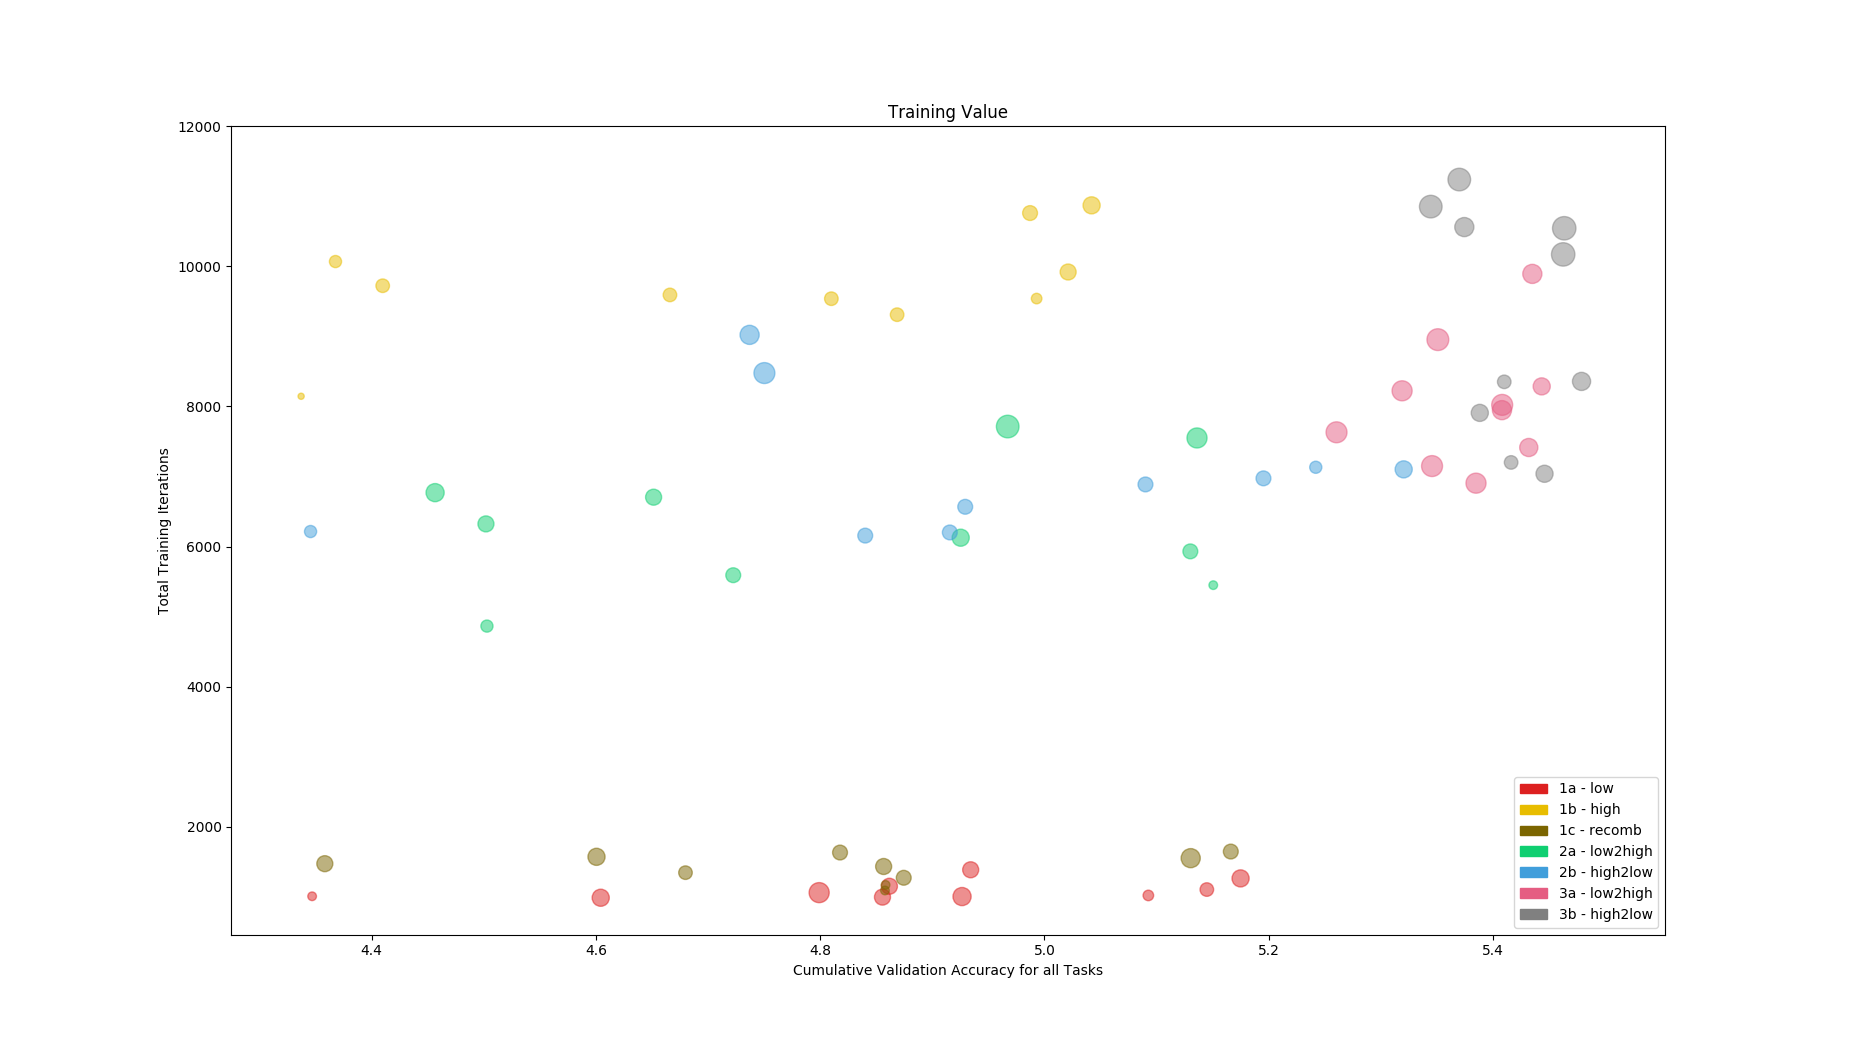
\includegraphics[width=\textwidth]{Chapters/Experiments/search_algo/figures/Training_value.png}
    \caption{}
    \label{fig:search.training_value}
\end{figure}

\begin{figure}[h]
    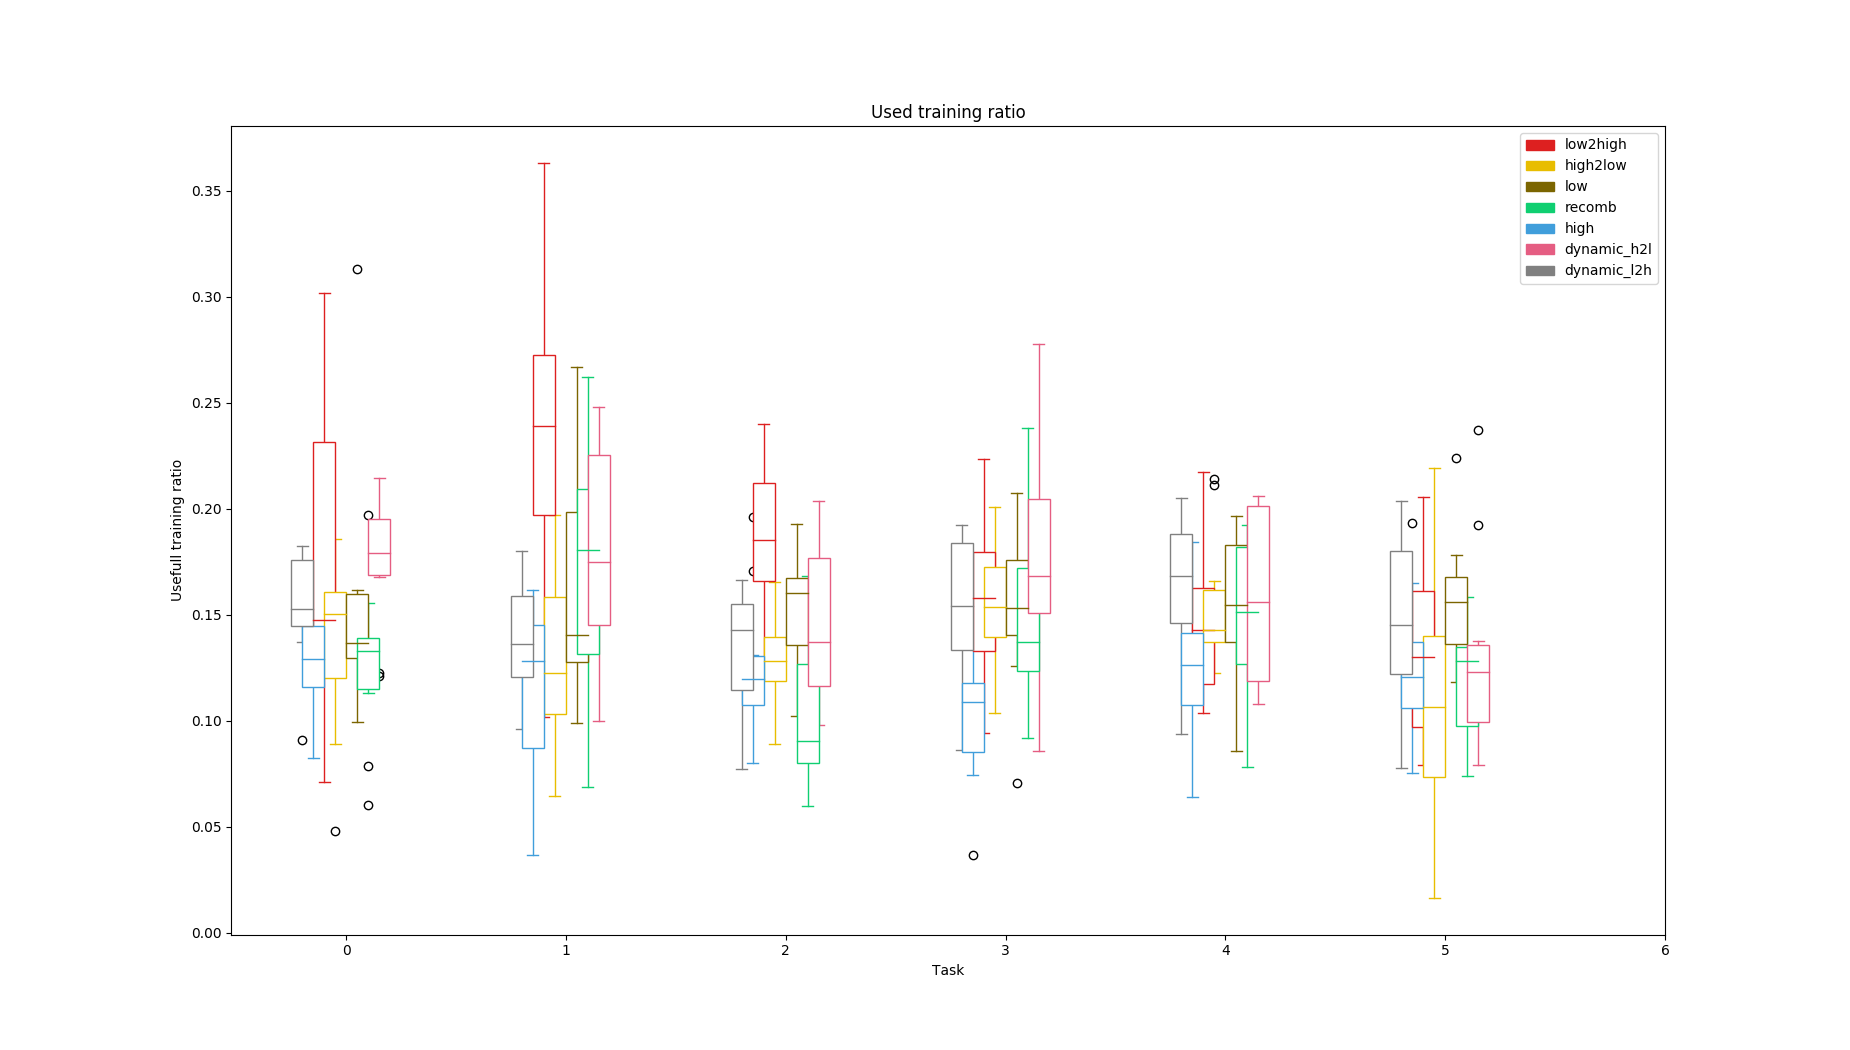
\includegraphics[width=\textwidth]{Chapters/Experiments/search_algo/figures/Used_training_ratio.png}
    \caption{}
    \label{fig:search.usefull_training}
\end{figure}

\section{Discussion}
\section{Conclusion}